\documentclass[8pt,a4]{extarticle}
\usepackage{multicol,caption}
\usepackage[utf8]{inputenc}
\usepackage[italian]{babel}
\usepackage[a4paper, landscape, margin=1cm, footskip=0.7cm]{geometry}
\usepackage{graphicx}
\usepackage{lipsum}
\usepackage{amsmath}
\usepackage{dsfont}
\usepackage{gensymb}
\usepackage{mathrsfs}
\usepackage{framed}
\usepackage{enumerate}
\usepackage{array}
\usepackage{datetime}
\usepackage{calligra}
\usepackage[dvipsnames]{xcolor}
\usepackage[titles]{tocloft}
\usepackage[sfdefault]{roboto}
\usepackage{enumitem}
\usepackage[titles]{tocloft}

\setenumerate{itemsep=0.2pt,topsep=3pt}
\setitemize{itemsep=0.2pt, topsep=3pt}

\graphicspath{{figures/}}

\newenvironment{Figure}
  {\par\medskip\noindent\minipage{\linewidth}}
  {\endminipage\par\medskip}

\newenvironment{conditions}
{\par\vspace{\abovedisplayskip}\noindent\begin{tabular}{>{$}l<{$} @{${}={}$} l}}
{\end{tabular}\par\vspace{\belowdisplayskip}}

\setlength{\columnseprule}{0.2pt}
\setlength{\columnsep}{10pt}
\renewcommand{\columnseprulecolor}{\color{lightgray}}

% TOC
\setlength{\cftbeforesecskip}{-.2ex}

\begin{document}

\begin{multicols}{3}
\noindent
\large IT Systems Management
\normalsize \\
\today, \currenttime
\vspace{-1.2em}\\
\tableofcontents
\columnbreak
\section{Executive Support} 
Crucial for SysMan. Business metrics is a good argument for Ex. Supp., continuous support
should be ensured. \\

\section{Organizing for Systems Management}
\subsection{Factors to Consider in Designing IT Organizations}
In the case of IT, restructuring is often necessary to support company growth, increased customer demand, 
changing business requirements, acquisitions, mergers, buyouts, or other industry changes.
Three key factors by which infrastructures can be organized: 
departmental responsibilities, planning orientation, and systems management processes.
\paragraph{Org. Model} Know Your Business (KYB), Locating Deparments in the Infrastructure, Identify Process Owners.

\section{Staffing for System Management}
Skilled professionals are needed at the outset to develop plans, design processes, and evaluate technologies; 
then they are needed to transform these ideas from paper into realities.

\paragraph{Skill Set} defined as technical familiarity with a particular software product, architecture, or platform.
\paragraph{Skill Level} defined as the length of experience and depth of technical expertise and variety of platform
familiarity an individual has acquired and can apply to a given technology.

\paragraph{Importance of the right staff} Determining required skill sets and skills levels, assessing skill levels of
current onboard staff (alternative sources of staffing, recruiting infra. staff from 
the outside [operative/consultive]), selecting the \textit{Most Qualified Candidate},
retaining \textit{Key Personnel}, using \textit{Consultants and Contractors} 
(benefits / drawbacks are involved, steps for developing career paths for staff memebers)

\section{Ethics, Legislation, and Outsourcing}
\paragraph{Personal Ethics} Set values an individual uses to influence and guide his or her personal behavior.
\paragraph{Business Ethics} Set values an individual uses to influence and guide his or her business behavior.
Business ethics tend to focus on the behaviors of an individual as it pertains to his or her work environment.
The differences between personal and business ethics may be at once both subtle and far-reaching.

\paragraph{NPI} Stands for non-public information and pertains to the private, 
personal information of an individual not readily available in public records. 
Customers typically disclose such information to private or public companies to transact business. 
Examples of NPI are social security numbers, unlisted telephone numbers, and credit card account numbers.

\section{Customer Service}
IT evolved into a service organization. 
\begin{itemize}
\item Identifying your key customers
\item Identifying key services of key customers
\item Identifying key processes that support key services
\item Identifying key suppliers that support key processes
\end{itemize}
Integrating the 4 key elements of Good Customer Service.
\section{Availability}
\paragraph{Availability} Process of optimizing the readiness of production systems by accurately
 measuring, analyzing, and reducing outages to those production systems. \\
{\tiny The ratio of the {\color{MidnightBlue}{total time a functional unit is capable of being
 used during a given interval}} to {\color{MidnightBlue}{the length of the interval}}. \\
Mean Time To Failure (MTTF), Mean Time To Repair (MTTR)}
\paragraph{Responsiveness} Operational responsiveness is a quality of a business process or supporting IT solution, 
which indicates its ability to respond to changing conditions and customer interactions as they occur.  
\paragraph{Uptime} measure of the time that individual components within a production system are functionally operating.
This contrasts to availability, which focuses on the production system as a whole.

\paragraph{Slow Response} refers to unacceptably long periods of time for an online transaction to complete processing 
and return results to the user. 
The period of time deemed unacceptable varies depending on the type of transaction involved. 
For simple inquiries, a one-second response may seem slow; for complex computations, 
two- or three-second responses may be acceptable. Slow response is usually a performance and tuning problem requiring 
highly-trained personnel with specialized expertise

\paragraph{Downtime} Downtime refers to the total inoperability of a hardware device, a software routine, or some other
critical component of a system that results in the outage of a production application.

\paragraph{High Availability} refers to the design of a production environment such that all single points of failure 
are removed through redundancy to eliminate production outages. 
This type of environment is often referred to as being fault tolerant.

\paragraph{SMART} \textbf{S}pecific, \textit{Targets should be straightforward and emphasize what you want to happen}.
\textbf{M}easurable, \textit{If a target cannot be measured then you cannot determine whether it has been
achieved}. \textbf{A}chievable, \textit{It must be possible to achieve the target with an acceptable investment of time
and resources}. \textbf{R}elevant, \textit{Achieving the target must contribute to the overall business mission}.
\textbf{T}imely, \textit{The target must be something that can be achieved and measured over the
reporting period of the SLA\footnote{SLA is short for service level agreement and refers to a documented, 
negotiated agreement between a representative from an IT department and a representative from an end-user department 
concerning the quality of service delivered. 
Common SLA metrics include percent uptime availability, average response times, 
and escalation procedures for problems.}}.

\subsection{7-R{\small s} of availability}
These seven Rs of high availability all contribute in a unique way to extending uptime, minimizing downtime,
and improving the overall level of service provided by online systems.

\subsubsection{Redundancy}
Power Supply, Multiple processors, Segmented Memory, Redundant Disks
\subsubsection{Reputation}
The reputation of key suppliers of servers, disk storage systems, database management systems, and network hardware and
software plays a principle role in striving for high availability.
It is always best to go with the best. Reputations can be verified in several ways, including the following: Percent 
of market share, Reports from industry analysts such as Gartner Group, Publications such Wall Street Journal and
ComputerWorld, Track record of reliability and repairability, Customer references

\subsubsection{Reliability}
The reliability of the hardware and software can also be verified from customer 
references and industry analysts. 
Beyond that, you should consider performing what we call an empirical component reliability analysis.
The following list describes the seven steps required to accomplish this.

\begin{enumerate}
    \item Review and analyze problem management logs.
    \item Review and analyze supplier logs.
    \item Acquire feedback from operations personnel.
    \item Acquire feedback from support personnel.
    \item Acquire feedback from supplier repair personnel.
    \item Compare experiences with other shops.
    \item Study reports from industry analysts.
\end{enumerate}


\subsubsection{Repairability}
This refers to is the relative ease with which service technicians can resolve or replace failing components. 
A common metric used to evaluate this trait is the average or mean time to repair (MTTR).
MTTR is sometimes interpreted as the mean time to recover, the mean time to restore, or the mean time to resolve. 
It measures the average time it takes to do the actual repair.
$\text{MTTR} = \frac{\text{sum of repair times}}{\text{\# of failures}}$
\subsubsection{Recoverability}
This refers to the ability to overcome a momentary failure in such a way that there is no impact on end-user 
availability. 
It could be as small as a portion of main memory recovering from a single-bit memory error; 
it can be as large as having an entire server system switch over to its standby system with no loss of data or 
transactions. 
Recoverability also includes retries of attempted reads and writes out to disk or tape, as well as the retrying of 
transmissions down network lines.
\subsubsection{Responsiveness}
This trait is the sense of urgency all people involved with high availability need to exhibit. 
This includes having well-trained suppliers and in-house support personnel who can respond to problems quickly and 
efficiently. 
It also pertains to how quickly the automated recovery of resources such as disks or servers can be enacted.
Escalation is another aspect of responsiveness that ensures higher levels of technical expertise and management support
are involved to restore availability as quickly as possible. 
Escalation guidelines are usually documented in service-level agreements between IT and business customers.

\subsubsection{Robustness}
A robust process will be able to withstand a variety of forces—both internal and external—that could easily disrupt 
and undermine availability in a weaker environment. 
Robustness puts a high premium on documentation and training to withstand the following:
\paragraph{Technical Changes as they relate to} Platforms, Products, Services, Customers
\paragraph{Personnel Changes as they relate to} Turnover, Expansion, Rotation
\paragraph{Business changes as they relate to} New direction, Acquisitions, Mergers

Defining a process to measure and monitor Infrastructure's Availability: Committed Hours of Availability (A),
Outage hours (B), Achieved Availability: $\frac{A-B}{A} \cdot 100 \%$.

\section{Performance and Tuning}
Methodology to maximize throughput and minimize response times of batch jobs,
online transactions, and Internet activities.
The five infrastructure areas most impacted by performance and tuning are:
\begin{itemize}
    \item Servers
    \item Disk storage
    \item Databases
    \item Networks
    \item Desktop Computers
\end{itemize}
\section{Production Acceptance}
Methodology used to consistently and successfully deploy application systems into a 
production environment regardless of platform.

\paragraph{Consistent methodology} While the methodology is consistent, it is not necessarily identical across all 
platforms. This means there are essential steps of the process that need to be done for every production deployment, 
and then there are other steps that can be added, omitted, or modified depending on the type of platform selected 
for production use.
 
\paragraph{Deploying into a production environment} This implies that the process is not complete until all users are 
fully up and running on the new system. For large applications, this could involve thousands of users phased in over
several months.
 
\paragraph{Application system} This refers to any group of software programs necessary for conducting a company’s
business—the end-users of which are primarily, but not necessarily, in departments outside of IT. 
This excludes software still in development, as well as software used as tools for IT support groups.

\paragraph{Production Acceptance Process}
\begin{enumerate}
\item Identify an Executive Sponsor
\item Select a Process Owner
\item Solicit Executive Support
\item Assemble a Production Acceptance Team
\item Identify and Prioritize Requirements
\item Develop Policy Statements
\item Nominate a Pilot System
\item Design Appropriate Forms
\item Document updates, extension and new procedures
\item Run field tests and a solid pilot phase
\item Revise Policies, Procedures, and Forms
\item Define an adequate marketing strategy (if applicable)
\item Conduct a lessons-learned sessions
\item Follow-up with continuous improvements
\end{enumerate}
\noindent
Pay attention:
\begin{itemize}
\item Production Acceptance is not Change Management
\item New Applications vs. New Versions of Existing Applications
\end{itemize}

\section{Change Management}
Change Management is the process to control and coordinate all changes to an IT production environment. 
Control involves requesting, prioritizing, and approving changes; coordination involves collaborating, scheduling,
communicating, and implementing changes. \\
A change is defined as any modification that could impact the stability or responsiveness of an
IT production environment.

\subsection{Key Steps Required in Developing a Change Management Process}
\begin{enumerate}
\item Identify an executive sponsor.
\item Assign a process owner.
\item Select a cross-functional process design team.
\item Arrange for meetings of the cross-functional process design team.
\item Establish roles and responsibilities for members supporting the design team.
\item Identify the benefits of a change management process.
\item If change metrics exist, collect and analyze them; if not, set up a process to do so.
\item Identify and prioritize requirements.
\item Develop definitions of key terms.
\item Design the initial change management process.
\item Develop policy statements.
\item Develop a charter for a Change Advisory Board (CAB).
\item Use the CAB to continually refine and improve the change management process.
\end{enumerate}

\subsection{Tasks in the scope of CMP}
\begin{itemize}
\item SDLC – Changes handled through the formal software development life cycle will be included within the 
company’s change management program.
\item Hardware – Installation, modification, removal or relocation of computing equipment.
\item Software – Installation, patching, upgrade or removal of software products including operating systems, access methods, commercial off-the-shelf (COTS) packages, internally developed packages and utilities.
\item Database – Changes to databases or files such as additions, reorganizations and major maintenance.
\item Application – Application changes being promoted to production as well as the integration of new application systems and the removal of obsolete elements.
\item Moves, Adds, Changes and Deletes – Changes to system configuration.
\item Scheduled Changes - Requests for creation, deletion, or revision to job schedules, back-up schedules or other regularly scheduled jobs managed by the IT department.
\item Telephony – Installation, modification, de-installation, or relocation of PBX/VOIP equipment and services.
\item Desktop – Any modification or relocation of desktop equipment and services for users or classroom labs.
\item Generic and Miscellaneous Changes – Any changes that are required to complete tasks associated with normal job requirements.
\end{itemize}

\subsection{Tasks that aren't part of CMP}
\begin{itemize}
\item Contingency/Disaster Recovery
\item BCM related activities
\item Changes to non-production elements or resources
\item Changes made within the daily administrative process.
\begin{itemize}
\item Password resets
\item User adds/deletes
\item User modifications
\item Adding, deleting or revising security groups
\item Rebooting machines when there is no change to the
\item configuration of the system
\item File permission changes
\end{itemize}
\end{itemize}

\section{Problem Management}
Problem management is a process used to identify, log, track, resolve, and analyze problems impacting IT services.

\subsection{Scope of Problem Management}
Many infrastructures do agree that first-level problem handling, commonly referred to as tier 1,
 is the minimum basis for problem management.

\subsection{Key Steps to Developing a Problem Management Process}
\begin{enumerate}
\item Select an executive sponsor.
\item Assign a process owner.
\item Assemble a cross-functional team.
\item Identify and prioritize requirements.
\item Establish a priority and escalation scheme.
\item Identify alternative call-tracking tools.
\item Negotiate service levels.
\item Develop service and process metrics.
\item Design the call-handling process.
\item Evaluate, select, and implement the call-tracking tool.
\item Review metrics to continually improve the process.
\end{enumerate}

\section{Storage Management}
Storage management is a process used to optimize the use of storage devices and to protect the integrity of data 
for any media on which it resides.

\subsection{Storage Management Capacity}
Storage management capacity consists of providing sufficient data storage to authorized users at a reasonable cost.

\subsection{Storage Management Performance}
The first performance consideration is the size and type of main memory.

\subsection{Storage Management Reliability}
Fault tolerance w/ RAID Systems

\resizebox{0.8\columnwidth}{!}{
    \begin{minipage}[t][][b]{\columnwidth}
        \centering
\begin{tabular}{|l|l|}
    \hline
    \textbf{RAID Level} & \textbf{Explanation} \\\hline
    0 & Disk striping for performance \\\hline
    1 & Mirroring for total redundancy \\\hline
    0 + 1 & Combination of striping and mirroring \\\hline
    3 & Striping and fault tolerance with parity on totally dedicated parity drives \\\hline
    5 & Striping and fault tolerance with parity on nonassociated data drives \\\hline 
\end{tabular}
\end{minipage}
}

\subsection{Storage Management Recoverability}
several methods available for recovering data that has been altered, deleted, damaged, or otherwise made inaccessible.
Determining the correct recovery technique depends on the manner in which the data was backed up.

\section{Network Management}
Process to maximize the reliability and utilization of network components in order to optimize network availability 
and responsiveness.


\subsection{Key Decisions about Network Management}
\begin{enumerate}
\item What will be managed by this process?
\item Who will manage it?
\item How much authority will this person be given?
\item What types of tools and support will be provided?
\item To what extent will other processes be integrated with this process?
\item What levels of service and quality will be expected?
\end{enumerate}

\subsection{Assessing an Infrastructure’s Network Management Process}
\subsection{Measuring and Streamlining the Network Management Process}
We can measure the effectiveness of a network management process with service metrics such as network availability, 
network response times, and elapsed time to logon.

\section{Configuration Management}
Process to ensure that the interrelationships of varying versions of infrastructure hardware and software are
documented accurately and efficiently. \\
\\
Configuration management refers to coordinating and documenting the different levels of hardware, firmware, and 
software that comprise mainframes, servers, desktops, databases, and various network devices such as routers, hubs,
and switches. It does not refer to application software systems or to the verification of various levels of application
software in different stages of development, testing, and deployment—these activities are commonly referred to as
versioning control and are normally managed by the applications development group or by a software quality assurance 
group within applications development.

\subsection{Pratical Tips for Improving Config. Man.}
\begin{enumerate}
    \item Select a qualified process owner.
    \item Acquire the assistance of a technical writer or a documentation analyst.
    \item Match the backgrounds of writers to technicians.
    \item Evaluate the quality and value of existing configuration documentation.
    \item Involve appropriate hardware suppliers.
    \item Involve appropriate software suppliers.
    \item Coordinate documentation efforts in advance of major hardware and software upgrades.
    \item Involve the asset-management group for desktop equipment inventories.
\end{enumerate}

\subsection{Assessing an Infrastructure’s Configuration Management Process}
% ?????
\subsection{Measuring and Streamlining the Configuration Management Process}
We can measure the effectiveness of a configuration management process with service metrics such as the number of times
analysts, auditors, or repair technicians find out-of-date configuration documentation. 
Process metrics, such as the elapsed time between altering the physical or logical configuration and noting it on 
configuration diagrams, help us gauge the efficiency of this process. 
And we can streamline the configuration management process by automating certain actions—the updating of multiple 
pieces of documentation requiring the same update, for example.

\section{Cloud Services}
\subsection{Characteristics of a Cloud}
\begin{itemize}
\item Resource pooling is the most fundamental characteristic, as discussed above. The
provider abstracts resources and collects them into a pool, portions of which can be
allocated to different consumers (typically based on policies).
\item Consumers provision the resources from the pool using on-demand self-service.
They manage their resources themselves, without having to talk to a human
administrator.
\item Broad network access means that all resources are available over a network,
without any need for direct physical access; the network is not necessarily part of
the service.
\item Rapid elasticity allows consumers to expand or contract the resources they use
from the pool (provisioning and deprovisioning), often completely automatically. This
allows them to more closely match resource consumption with demand (for
example, adding virtual servers as demand increases, then shutting them down
when demand drops).
\item Measured service meters what is provided, to ensure that consumers only use what
they are allotted, and, if necessary, to charge them for it. This is where the term
utility computing comes from, since computing resources can now be consumed like
water and electricity, with the client only paying for what they use.
\end{itemize}

\subsection{Cloud Services}
\begin{itemize}
\item Software as a Service (SaaS) is a full application that’s managed and
hosted by the provider. Consumers access it with a web browser,
mobile app, or a lightweight client app.
\item Platform as a Service (PaaS) abstracts and provides development or
application platforms, such as databases, application platforms (e.g. a
place to run Python, PHP, or other code), file storage and
collaboration, or even proprietary application processing (such as
machine learning, big data processing, or direct Application
Programming Interfaces (API) access to features of a full SaaS
application). The key differentiator is that, with PaaS, you don’t
manage the underlying servers, networks, or other infrastructure.
\item Infrastructure as a Service (IaaS) offers access to a resource pool of
fundamental computing infrastructure, such as compute, network, or
storage.
\end{itemize}

\section{Capacity Planning}
As its name implies, the systems management discipline of capacity planning involves the planning of various kinds
of resource capacities for an infrastructure. \\
Capacity planning is a process to predict the types, quantities, and timing of critical resource capacities that are 
needed within an infrastructure to meet accurately forecasted workloads.\\
\subsection{4 Key Elements}
\begin{enumerate}
    \item The type of resource capacities required, such as servers, disk space, or bandwidth
    \item The size or quantities of the resource in question
    \item The exact timing of when the additional capacity is needed
    \item Decisions about capacity that are based on sound, thorough forecasts of anticipated workload demands
\end{enumerate}

\subsection{Why Capacity Planning Is Seldom Done Well}
\begin{enumerate}
    \item Analysts Are Too Busy with Day-To-Day Activities
    \item Users Are Not Interested (or able?) in Predicting Future Workloads
    \item Users Who Are Interested Cannot Forecast Accurately
    \item Capacity Planners May Be Reluctant to Use Effective Measuring
    Tools
    \item Need for updates: Corporate or IT Directions May Change over
    time (e.g. yearly)
    \item Planning Is Typically Not Part of an Infrastructure Culture
    \item Managers Sometimes Confuse Capacity Management with Capacity Planning
\end{enumerate}

\subsection{Steps to develop an effective capacity planning process}
\begin{enumerate}
    \item Select an Appropriate Capacity Planning Process Owner
    \item Identify the Key (Critical?) Resources to be Measured
    \item Monitor the Utilizations or Performance of the Resources
    \item Compare Utilizations to Maximum Capacities
    \item Collect Workload Forecasts from Developers and Users
    \item Transform Workload Forecasts into IT Resource Requirements
    \item Map Requirements onto Existing Utilizations
    \item Predict When the Business/Company Will Be Out of Capacity
    \item Update Forecasts and Utilizations
\end{enumerate}

\subsection{Additional Benefits of Capacity Planning}
\begin{enumerate}
    \item Strengthens Relationships with Developers and End-Users
    \item Improves Communications with Suppliers
    \item Encourages Collaboration with Other Infrastructure Groups
    \item Promotes a Culture of Strategic Planning as Opposed to Tactical Firefighting
\end{enumerate}

\subsection{Helpful Hints for Effective Capacity Planning}
\begin{enumerate}
    \item Start Small
    \item Speak the Language of Your Customers
    \item Consider Future Platforms
    \item Share Plans with Suppliers
    \item Anticipate Nonlinear Cost Ratios
    \item Plan for Occasional Workload Reductions
    \item Prepare for the Turnover of Personnel
    \item Strive to Continually Improve the Process
    \item Evaluate the Hidden Costs of Upgrades
\end{enumerate}

\subsection{Uncovering the Hidden Costs of Upgrades}
\begin{enumerate}
    \item Hardware Maintenance
    \item Technical Support
    \item Software Maintenance
    \item Memory Upgrades
    \item Channel Upgrades
    \item Cache Upgrades
    \item Data Backup Time
    \item Operations Support
    \item Offsite Storage
    \item Network Hardware
    \item Network Support
    \item Floor Space
    \item Power and Air Conditioning
\end{enumerate}

\subsection{Assessing an Infrastructure’s Capacity Planning Process}
\subsection{Measuring and Streamlining the Capacity Planning Process}
We can measure the effectiveness of a capacity planning process with service metrics such as the number of instances of 
poor response due to inadequate capacity on servers, disk devices, or the network. 
Process metrics—such as the number of instances of poor response due to inadequate capacity on servers, disk devices, 
or the network—help us gauge the efficiency of this process. 
We can be streamline the capacity planning process by automating certain actions—the notification to analysts when 
utilization thresholds are exceeded, the submittal of user forecasts, and the conversion of user-workload forecasts 
into capacity requirements, for example.

\section{Strategic Security}
Strategic security is designed to safeguard the availability, integrity, and confidentiality of designated data
 and programs against unauthorized access, modification, or destruction.

\subsection{Developing a Strategic Security Process}
\begin{enumerate}
    \item Identify an executive sponsor.
    \item Select a process owner.
    \item Define goals of strategic security.
    \item Establish review boards.
    \item Identify, categorize, and prioritize requirements.
    \item Inventory current state of security.
    \item Establish security organization.
    \item Develop security policies.
    \item Assemble planning teams.
    \item Review and approve plans.
    \item Evaluate technical feasibility of plans.
    \item Assign and schedule the implementation of plans.
\end{enumerate}

\subsection{Measuring and Streamlining the Security Process}
We can measure the effectiveness of a security process with service metrics such as the number of outages caused by 
security breaches and the amount of data altered, damaged, or deleted due to security violations. 
Process metrics, such as the number of password resets requested and granted and the number of multiple sign-ons 
processed over time, help us gauge the efficiency of this process. 
Finally, we can streamline the security process by automating certain actions—for example, the analysis of password 
resets, network violations, or virus protection invocations.

\section{Business Continuity}
Business continuity is a methodology to ensure the continuous operation of critical business systems in the event
of widespread or localized disasters to an infrastructure environment.

\subsection{Steps to Developing an Effective Business Continuity Process}
\begin{enumerate}
    \item Acquire executive support.
    \item Select a process owner.
    \item Assemble a cross-functional team.
    \item Conduct a business impact analysis.
    \item Identify and prioritize requirements.
    \item Assess possible business continuity recovery strategies.
    \item Develop a request for proposal (RFP) for outside services.
    \item Evaluate proposals and select the best offering.
    \item Choose participants and clarify their roles on the recovery team.
    \item Document the business continuity plan.
    \item Plan and execute regularly scheduled tests of the plan.
    \item Conduct a lessons-learned postmortem after each test.
    \item Continually maintain, update, and improve the plan.
\end{enumerate}

\section{Facilities Management}
Facilities management is a process to ensure that an appropriate physical environment is consistently supplied to 
enable the continuous operation of all critical infrastructure equipment.
\subsection{Major Elements}
\paragraph{UPS} uninterruptible power supply and is a temporary battery backup in the event of commercial power loss.
UPS units are normally used to power data centers for 15-20 minutes until such time that commercial power is restored 
or until longer term backup generators come online. 
Portable UPS units are now available for servers, workstations and desktops outside of a data center.

\subsection{Facilities Management Process Owner}
\begin{itemize}
    \item Determining the Scope of Responsibilities of a Facilities Management Process Owner
    \item Desired Traits of a Facilities Management Process Owner
\end{itemize}
The owner of the facilities management process almost always resides in the computer operations department.

\subsection{Evaluating the Physical Environment}
\begin{itemize}
    \item Major Physical Exposures Common to a Data Center
    \item Keeping Physical Layouts Efficient and Effective
\end{itemize}
If the problem-management system includes a robust database, it should be easy to analyze trouble tickets caused by 
facilities issues and highlight trends, repeat incidents, and root causes.

\subsection{Tips to Improve the Facilities Management Process}
\begin{enumerate}
    \item Nurture relationships with facilities department.
    \item Establish relationships with local government inspecting agencies, 
        especially if you are considering major physical upgrades to the data center.
    \item Consider using video cameras to enhance physical security.
    \item Analyze environmental monitoring
        reports to identify trends, patterns, and relationships.
    \item Design adequate cooling for hot spots due to concentrated equipment.
    \item Check on effectiveness of water and fire detection and suppression systems.
    \item Remove all tripping hazards in the computer center.
    \item Check on earthquake preparedness of data center
        (devices anchored down, training of personnel, and tie-in to disaster recovery).
\end{enumerate}
\subsection{Facilities Management at Outsourcing Centers}
Shops that outsource portions of their infrastructure services—co-location of servers is an example—often feel that the 
responsibility for the facilities management process is also outsourced and no longer of their concern. 
While outsourcers have direct responsibilities for providing stable physical environments, the client has an 
indirect responsibility to ensure this will occur. 
During the evaluation of bids and in contract negotiations, appropriate infrastructure personnel should ask the same 
types of questions about the outsourcer’s physical environment that they would ask if it were their own computer center.
\subsection{Measuring and Streamlining the Facilities Management Process}
We can measure the effectiveness of a facilities management process with service metrics such as the number 
of outages due to facilities management issues and the number of employee safety issues measured over time. 
Process metrics—for example, the frequency of preventative maintenance and inspections of air conditioning, 
smoke detection, and fire suppression systems and the testing of uninterruptible power supplies and backup 
generators—help us gauge the efficiency of this process. And we can streamline the facilities management process by 
automating actions such as notifying facilities personnel when environmental monitoring thresholds are exceeded 
for air conditioning, smoke detection, and fire suppression.

\section{IT Monitoring}
\begin{center}
\begin{minipage}[t][4cm][b]{4cm}
    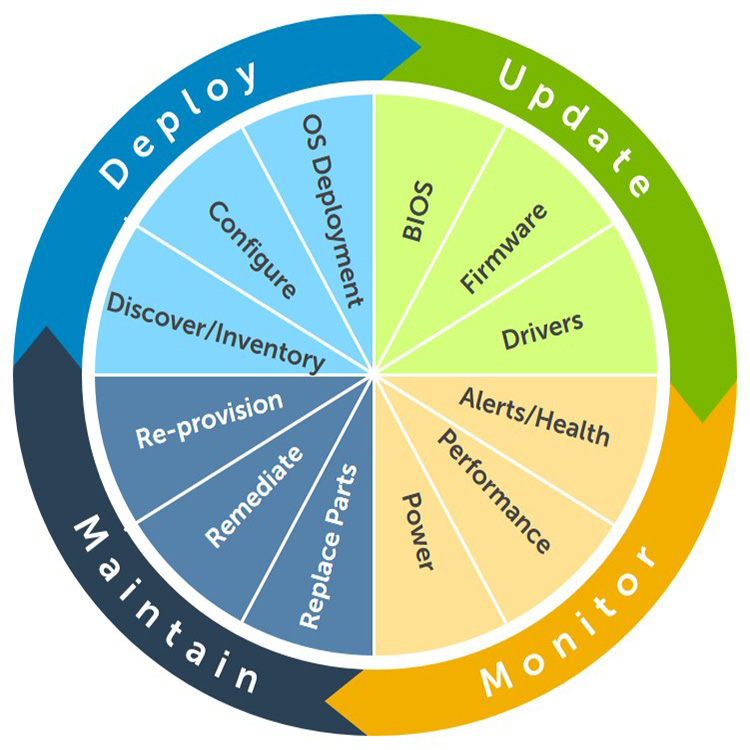
\includegraphics[height=4cm]{dell-lc-management.jpg}
\end{minipage}
\end{center}

Monitoring Priorities for Systems Management
\begin{itemize}
    \item Operating System Performance and Availability
    \item Server Hardware Status
    \item Data and Storage Availability
    \item Directory Services
    \item Patches and Updates
    \item Virtualization Infrastructure Performance
    \item Problem and Incident Alarming and Reporting
    \item Change Detection and Behavioral analysis
    \item Capacity Planning
    \item Email Server Monitoring
\end{itemize}

\subsection{80\% Rule}
When servers regularly exceed about 80\% of their capacity – in terms of CPU utilization, memory performance, 
and storage availability – they should be upgraded or replaced. 

\section{CoBIT Framework}
\begin{center}
    \begin{minipage}[t][4cm][b]{4cm}
        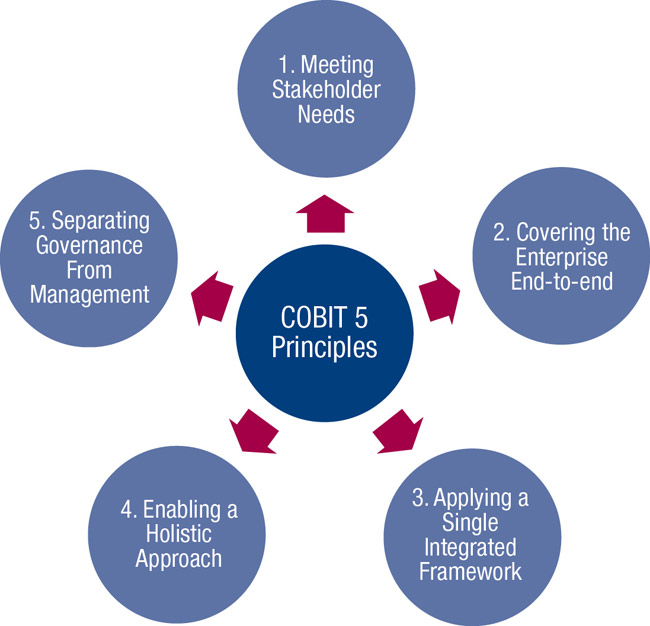
\includegraphics[height=4cm]{cobit-fw.jpg}
    \end{minipage}
\end{center}
\noindent
The COBIT 5 framework defines
7 categories of enablers:
\begin{itemize}
    \item Principles, Policies and Frameworks
    \item Processes
    \item Organisational Structures
    \item Culture, Ethics and Behaviour
    \item Information
    \item Services, Infrastructure and Applications
    \item People, Skills and Competencies
\end{itemize}
\vspace{1em}
\noindent
The COBIT 5 framework makes a clear distinction between
governance and management. These two disciplines encompass
different types of activities, require different organisational structures
and serve different purposes. COBIT 5’s view on this key distinction
between governance and management is:

\begin{itemize}
    \item Governance ensures that stakeholder needs, conditions and options
    are evaluated to determine balanced, agreed-on enterprise objectives
    to be achieved; setting direction through prioritisation and decision
    making; and monitoring performance and compliance against
    agreed-on direction and objectives (e.g. board of directors).
    \item Management plans, builds, runs and monitors activities in alignment
    with the direction set by the governance body to achieve the
    enterprise objectives (e.g. CEO).
\end{itemize}

\subsection{ISACA}
Leading global provider of knowledge, certifications, community, advocacy, education on information systems (IS), 
assurance and security, enterprise governance and management of IT, IT-related risk and compliance.\\
95,000 constituents in 160 countries. ISACA attests IT skills \& knowledge through recognized certifications:
\begin{itemize}
    \item Certified Information Systems Auditor® (CISA®),
    \item Certified Information Security Manager® (CISM®),
    \item Certified in the Governance of Enterprise IT® (CGEIT®) and
    \item Certified in Risk and Information Systems ControlTM (CRISCTM) designations
\end{itemize}

\subsection{CoBIT 5: SIEM}
Security information and event management (SIEM), it is a solution enterprise security professionals both insight into
and a track record of the activities within their IT environment. It provides Real time analysis of log and event data,
to provide: 
\begin{itemize}
    \item threat monitoring,
    \item event correlation and
    \item incident response
\end{itemize}
\noindent
Collects and aggregates log data generated throughout the
organization’s technology infrastructure:
\begin{itemize}
    \item servers
    \item host systems
    \item applications
    \item network and
    \item security devices such as firewalls and antivirus filters.
\end{itemize}

SIEM software identifies and categorizes incidents and events, as well as analyzes them. \\
SIEM has 2 main objectives:
\begin{itemize}
    \item providing reports on security-related incidents and events,
    such as successful and failed logins, malware activity and
    other possible malicious activities
    \item sending alerts if the event analysis discovers an activity that
    runs against predetermined rulesets, indicating a potential
    security issue.
\end{itemize}

SIEM is implemented via software, systems, appliances, or some combination of these items. 
There are, generally speaking, six main attributes of an SIEM system:

\end{multicols}
\end{document}